% !TEX root = ../../../main.tex

\toggletrue{image}
\toggletrue{imagehover}
\chapterimage{the_search}
\chapterimagetitle{\uppercase{The Search}}
\chapterimageurl{https://xkcd.com/638/}
\chapterimagehover{"I am so excited about the Kepler mission. This is the second most important thing our species has ever done, right behind inventing the concept of delivery pizza."}

\chapter{Suchalgorithmen}
\label{chapter-suchalgorithmen}

Die Suche in Daten ist eine der grundlegendsten Operationen, die wir mit Computern durchführen wollen (z.B. die Suche nach einem Hashtag auf Instagram). Die Lernziele sind:

\newcommand{\suchalgorithmenLernziele}{
\protect\begin{todolist}
\item Sie definieren das Suchproblem für Zahlen.
\item Sie erklären das Prinzip der linearen und binären Suche.
\item Sie wenden einen Suchalgorithmus an.
\end{todolist}
}

\lernziel{\autoref{chapter-suchalgorithmen}, \nameref{chapter-suchalgorithmen}}{\protect\suchalgorithmenLernziele}

\suchalgorithmenLernziele

\vspace{-0.6cm}

\section{Grundlagen}

Wir können das Suchproblem für Zahlen wie folgt beschreiben:

\begin{problem}[Suchproblem]
Gegeben ist ein Array $A$ mit $n$ verschiedenen Zahlen. Eine gegebene Zahl $k$ soll im Array $A$ gesucht werden. Die Suche soll feststellen, ob die gegebene Zahl $k$ im Array vorhanden ist oder nicht.
\end{problem}

\begin{example}
	Kommt $42$ in $51$, $220$, $258$, $85$, $292$, $288$, $198$, $231$, $76$, $89$, $100$, $34$, $197$, $94$ vor?
\end{example}

\begin{definition}[Suchalgorithmus]
Ein Suchalgorithmus prüft, ob eine gegebene Zahl in einem gegebenen Array vorhanden ist oder nicht.
\end{definition}

\vspace{-0.6cm}

\section{Lineare Suche}

Der einfachste Suchalgorithmus ohne Vorbedingungen ist die \textbf{lineare Suche}.

\begin{lstlisting}[language={pseudocode}, caption={Lineare Suche.}, label={lst-algo-lineare-suche}]
input: Ein Array A mit n Zahlen, gesuchte Zahl k.
i $\gets$ 0
loop as long as i < n {
 if A[i] = k then {
  output: Suche erfolgreich
  stop
 }
 Erhöhe i um 1
}
output: Suche erfolglos
\end{lstlisting}

Die Idee der linearen Suche besteht darin, alle Zahlen des Arrays von vorne nach hinten durchzugehen und mit der gesuchten Zahl zu vergleichen. Die Suche kann \textbf{erfolgreich} beendet werden, sobald die Zahl \lstinline[language=pseudocode]{k} gefunden wurde. Dies wird durch die Anweisung \lstinline[language=pseudocode]{stop} in Zeile 5 von \autoref{lst-algo-lineare-suche} ausgedrückt. Das Prinzip der linearen Suche ist auch in \autoref{figure-linear-search} dargestellt.

\begin{figure}[htb]
\centering
\begin{minipage}{0.45\textwidth}
\centering
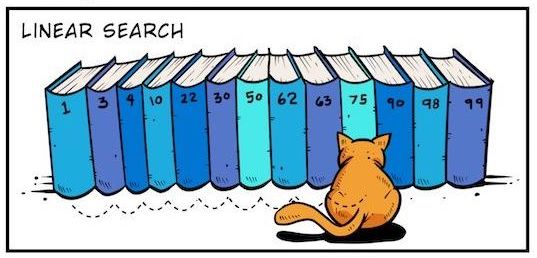
\includegraphics[width=\textwidth]{linear_search}
\caption{Wie finde ich ein Buch im \textbf{unsortierten} Bücherregal?}
\label{figure-linear-search}
\end{minipage}
\hfill
\begin{minipage}{0.45\textwidth}
\centering
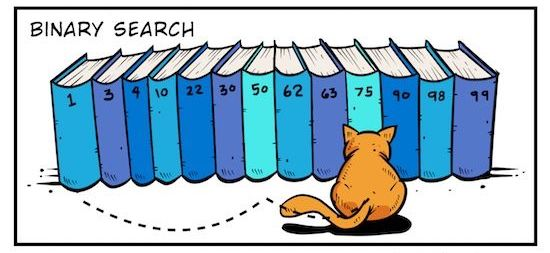
\includegraphics[width=\textwidth]{binary_search}
\caption{Wie finde ich ein Buch im Regal mit \textbf{sortierten} Bücherregal?}
\label{figure-binary-search}
\end{minipage}
\end{figure}

\section{Binäre Suche}

Wir passen nun die Voraussetzungen an und betrachten das Suchproblem erneut. Wir gehen jetzt davon aus, dass ein \textbf{sortiertes Array von Zahlen} gegeben ist.

\begin{example}
\lstinline[language=pseudocode]{[2, 12, 27, 42, 66, 101, 1024]} ist \textbf{aufsteigend}, \lstinline[language=pseudocode]{[65536, 8096, 1250,} \lstinline{50, 7, 0]} ist \textbf{absteigend} und \lstinline[language=pseudocode]{[1024, 8, 39, 40, 51} \lstinline{, 77]} ist \textbf{nicht} sortiert.
\end{example}

Nun lösen wir das Suchproblem erneut. Diesmal passen wir jedoch die Strategie an. Da das Array sortiert ist, beginnen wir mit dem Vergleich bei der \textbf{mittleren Zahl} des Arrays. Wenn die gesuchte Zahl nicht an dieser Position steht, prüfen wir, ob die gesuchte Zahl \textbf{kleiner} oder \textbf{grösser} als die \textbf{mittlere Zahl} ist. Auf diese Weise können wir \textbf{eine Hälfte} für die weitere Suche \textbf{ausschliessen}. In der \textbf{anderen Hälfte} suchen wir weiter und \textbf{wiederholen den Vorgang}. Wir bestimmen wieder die mittlere Zahl und vergleichen. Diese Schritte werden so lange wiederholt, bis wir ein Suchergebnis haben. \autoref{lst-algo-bin-suche} zeigt den Algorithmus der binären Suche. Das Prinzip der binären Suche ist ebenfalls in \autoref{figure-binary-search} dargestellt.

\begin{lstlisting}[language=pseudocode, caption={Binäre Suche (mit // in Code-Zeile 5 bedeutet ganzzahlige Division).}, label={lst-algo-bin-suche}]
input: Sortiertes Array A mit n Zahlen, gesuchte Zahl k.
indexLinks $\gets$ 0
indexRechts $\gets$ n - 1
loop as long as indexLinks $\leq$ indexRechts {
 indexMitte $\gets$ (indexLinks + indexRechts) // 2
 kandidat $\gets$ A[indexMitte]
 if kandidat = k then {
  output: Suche erfolgreich
  stop
 }
 elseif kandidat > k then {
  indexRechts $\gets$ indexMitte - 1
 }
 elseif kandidat < k then {
  indexLinks $\gets$ indexMitte + 1
 }
}
output: Suche erfolglos
\end{lstlisting}

Dieser Algorithmus ist komplizierter als die lineare Suche. Wir müssen die drei Fälle, \say{zu gross}, \say{zu klein} und \say{gleich} behandeln und die Indizes jeweils anpassen. \lstinline[language=pseudocode]{indexLinks} und \lstinline[language=pseudocode]{indexRechts} definieren jeweils einen Teil des Arrays, in dem gesucht wird. \lstinline[language=pseudocode]{indexMitte} wird für das Element verwendet, das mit der gesuchten Zahl verglichen werden soll.

\begin{example}[Ausführung binäre Suche]
\label{example-binary-search-k-12}
	Wir zeigen die binäre Suche Schritt-für-Schritt für das Array \lstinline[language=pseudocode]{A = [1, 3, 7, 8, 12, 21, 31]}. Gesucht wird die Zahl $k = 12$. Wir stellen das \textbf{Array als Tabelle} dar. \autoref{table-binary-search-bsp-01} zeigt die Ausgangssituation. Rot kennzeichnet den \lstinline{indexLinks}, blau den \lstinline{indexRechts} und grün den \lstinline{indexMitte}.

\begin{table}[H]
\centering
\begin{tblr}{
    colspec = {cccccccc},
    vline{2-Z} = {1}{solid}
}
\cline{2-8}
Element & 1 & 3 & 7 & 8 & 12 & 21 & 31 \\
\cline{2-8}
Index   & 0 & 1 & 2 & 3 & 4 & 5 & 6\\
\end{tblr}
\caption{Input: Array $A$ ($n = 7$) und gesuchte Zahl $k = 12$.}
\label{table-binary-search-bsp-01}
\end{table}

\begin{table}[htb]
\centering
\begin{minipage}[c]{0.45\textwidth}
\centering
\begin{tblr}{
    colspec = {cccccccc},
    vline{2-Z} = {1}{solid},
    cell{2}{2} = {red!25},
    cell{2}{8} = {green!25},
}
\cline{2-8}
Element & 1 & 3 & 7 & 8 & 12 & 21 & 31 \\
\cline{2-8}
Index   & 0 & 1 & 2 & 3 & 4 & 5 & 6\\
\end{tblr}
\caption{Stand nach Code-Zeile \num{3}.}
\label{table-binary-search-bsp-01}
\end{minipage}
\hfill
\begin{minipage}[c]{0.45\textwidth}
\centering
\begin{tblr}{
    colspec = {cccccccc},
    vline{2-Z} = {1}{solid},
    cell{2}{2} = {red!25},
    cell{2}{8} = {green!25},
    cell{2}{5} = {blue!25},
}
\cline{2-8}
Element & 1 & 3 & 7 & 8 & 12 & 21 & 31 \\
\cline{2-8}
Index   & 0 & 1 & 2 & 3 & 4 & 5 & 6\\
\end{tblr}
\caption{Stand \textbf{nach} Code-Zeile \num{5}.}
\label{table-binary-search-bsp-02}
\end{minipage}
\end{table}

Da die gesuchte Zahl ($k = 12$) \textbf{gösser} als $8$ ist, wird nun nur noch rechts von \lstinline{indexMitte} (blau) im Array gesucht. Deshalb wird nun der \lstinline{indexLinks} (rot) verschoben und im zweiten Schleifendurchlauf \lstinline{indexMitte} (blau) angepasst.

\begin{table}[H]
\centering
\begin{minipage}[c]{0.45\textwidth}
\centering
\begin{tblr}{
    colspec = {cccccccc},
    vline{2-Z} = {1}{solid},
    cell{2}{6} = {red!25},
    cell{2}{8} = {green!25},
    cell{2}{5} = {blue!25},
}
\cline{2-8}
Element & 1 & 3 & 7 & 8 & 12 & 21 & 31 \\
\cline{2-8}
Index   & 0 & 1 & 2 & 3 & 4 & 5 & 6\\
\end{tblr}
\caption{Stand nach Code-Zeile \num{15}.}
\label{table-binary-search-bsp-03}
\end{minipage}
\hfill
\begin{minipage}[c]{0.45\textwidth}
\centering
\begin{tblr}{
    colspec = {cccccccc},
    vline{2-Z} = {1}{solid},
    cell{2}{6} = {red!25},
    cell{2}{8} = {green!25},
    cell{2}{7} = {blue!25},
}
\cline{2-8}
Element & 1 & 3 & 7 & 8 & 12 & 21 & 31 \\
\cline{2-8}
Index   & 0 & 1 & 2 & 3 & 4 & 5 & 6\\
\end{tblr}
\caption{Stand \textbf{nach} Code-Zeile \num{5}.}
\label{table-binary-search-bsp-04}
\end{minipage}
\end{table}

Nun vergleichen wir wieder: $k = 12$ ist \textbf{kleiner} als $21$ (Zahl mit \lstinline{indexMitte} (blau)). Deshalb suchen wir jetzt links von \lstinline{indexMitte} (blau) bis zu \lstinline{indexLinks} (rot). Da es in diesem Bereich nur noch eine Zahl gibt, wird die Schleife diese Zahl beim \textbf{nächsten} Durchlauf finden.

\begin{table}[H]
\centering
\begin{minipage}[c]{0.45\textwidth}
\centering
\begin{tblr}{
    colspec = {cccccccc},
    vline{2-Z} = {1}{solid},
    cell{2}{6} = {red!25},
    cell{4}{6} = {green!25},
    cell{3}{7} = {blue!25},
}
\cline{2-8}
Element & 1 & 3 & 7 & 8 & 12 & 21 & 31 \\
\cline{2-8}
\lstinline{indexLinks}   & 0 & 1 & 2 & 3 & 4 & 5 & 6\\
\lstinline{indexMitte}   & 0 & 1 & 2 & 3 & 4 & 5 & 6\\
\lstinline{indexRechts}   & 0 & 1 & 2 & 3 & 4 & 5 & 6\\
\end{tblr}
\caption{Stand nach Code-Zeile \num{12}.}
\label{table-binary-search-bsp-05}
\end{minipage}
\hfill
\begin{minipage}[c]{0.45\textwidth}
\centering
\begin{tblr}{
    colspec = {cccccccc},
    vline{2-Z} = {1}{solid},
    cell{2}{6} = {red!25},
    cell{4}{6} = {green!25},
    cell{3}{6} = {blue!25},
}
\cline{2-8}
Element & 1 & 3 & 7 & 8 & 12 & 21 & 31 \\
\cline{2-8}
\lstinline{indexLinks}   & 0 & 1 & 2 & 3 & 4 & 5 & 6\\
\lstinline{indexMitte}   & 0 & 1 & 2 & 3 & 4 & 5 & 6\\
\lstinline{indexRechts}   & 0 & 1 & 2 & 3 & 4 & 5 & 6\\
\end{tblr}
\caption{Stand \textbf{nach} Code-Zeile \num{5}.}
\label{table-binary-search-bsp-06}
\end{minipage}
\end{table}

Da \lstinline{indexLinks} und \lstinline{indexRechts} gleich sind, führen wir die Schleife erneut aus. Wir aktualisieren \lstinline{indexMitte} (Code-Zeile $5$) und erhalten die \autoref{table-binary-search-bsp-06}. Dann führen wir erneut den Vergleich durch. Da $12$ ddie gesuchte Zahl ist, stoppt der Algorithmus bei Code-Zeile 9.
\end{example}

\section{Animation und Videomaterial}

Die Darstellung der binären Suche kann auf dem Papier schnell unübersichtlich werden. Ein Video bzw. eine Animation kann den Ablauf des Algorithmus eventuell besser zeigen.

\begin{itemize}
	\item Animation: \url{https://www.cs.usfca.edu/~galles/visualization/Search.html}
	\item Suchalgorithmen: \url{https://www.youtube.com/watch?v=7nI3qHAG8G4}
	\item Binäre Suche mit LEGO: \url{https://www.youtube.com/watch?v=Z1r2I2-TzU0}
\end{itemize}

\section{Übungen}

\begin{exercise}
Welche Algorithmen können benutzt werden, um im folgenden Array nach der Zahl \num{89} zu suchen? Begründen Sie Ihre Antwort.

\begin{center}
\lstinline[language=pseudocode]{A = [97, 67, 27, 25, 72, 7, 89, 59, 91, 98]}
\end{center}

\fillwithgrid{0.5in}

\end{exercise}

\begin{exercise}
Welche Algorithmen können benutzt werden, um im folgenden Array nach der Zahl \num{16} zu suchen? Begründen Sie Ihre Antwort.

\begin{center}
\lstinline[language=pseudocode]{A = [4, 8, 16, 20, 25, 35, 41, 56, 96, 97]}
\end{center}

\fillwithgrid{0.5in}

\end{exercise}

\begin{exercise}
Entwerfen Sie einen Algorithmus in Pseudocode für folgendes Problem. Tipp: Verwenden Sie den Pseudocode eines Suchalgorithmus als Grundlage.

\begin{problem}[Positionssuche-n-Zahlen]\label{problem-positionssuche-n-zahlen}
Es ist ein Array $A$ mit $n$ verschiedenen Zahlen und eine Zahl \lstinline[language=pseudocode]{k} gegeben. Die Positionssuche soll ermitteln, an welcher \textbf{Position} (Ausgabe soll der Index sein) die gegebene Zahl \lstinline[language=pseudocode]{k} vorhanden ist. Falls die Zahl \textbf{nicht} vorhanden ist, dann soll als Ausgabe für die Position \lstinline[language=pseudocode]{-1} verwendet werden.
\end{problem}

\fillwithgrid	{\stretch{1}}

\end{exercise}

\newpage

\begin{exercise}
\say{Spielen} Sie Computer und führen Sie die binäre Suche Schritt-für-Schritt aus. Stellen Sie den Ablauf wie in \autoref{example-binary-search-k-12} gezeigt dar.

\begin{enumerate}
\item \lstinline[language=pseudocode]{k = 7} \\
\begin{minipage}{0.45\textwidth}
\centering
\begin{tblr}{
    colspec = {cccccccc},
    vline{2-Z} = {1}{solid},
}
\cline{2-8}
Element & 1 & 3 & 7 & 8 & 12 & 21 & 31 \\
\cline{2-8}
Index   & 0 & 1 & 2 & 3 & 4 & 5 & 6\\
\end{tblr}
\end{minipage}
\hfill
\begin{minipage}{0.45\textwidth}
\centering
\begin{tblr}{
    colspec = {cccccccc},
    vline{2-Z} = {1}{solid},
}
\cline{2-8}
Element & 1 & 3 & 7 & 8 & 12 & 21 & 31 \\
\cline{2-8}
Index   & 0 & 1 & 2 & 3 & 4 & 5 & 6\\
\end{tblr}
\end{minipage}

\vspace{1cm}

\begin{minipage}{0.45\textwidth}
\centering	
\begin{tblr}{
    colspec = {cccccccc},
    vline{2-Z} = {1}{solid},
}
\cline{2-8}
Element & 1 & 3 & 7 & 8 & 12 & 21 & 31 \\
\cline{2-8}
Index   & 0 & 1 & 2 & 3 & 4 & 5 & 6\\
\end{tblr}
\end{minipage}
\hfill
\begin{minipage}{0.45\textwidth}
\centering
\begin{tblr}{
    colspec = {cccccccc},
    vline{2-Z} = {1}{solid},
}
\cline{2-8}
Element & 1 & 3 & 7 & 8 & 12 & 21 & 31 \\
\cline{2-8}
Index   & 0 & 1 & 2 & 3 & 4 & 5 & 6\\
\end{tblr}
\end{minipage}

\vspace{1cm}

\begin{minipage}{0.45\textwidth}
\centering	
\begin{tblr}{
    colspec = {cccccccc},
    vline{2-Z} = {1}{solid},
}
\cline{2-8}
Element & 1 & 3 & 7 & 8 & 12 & 21 & 31 \\
\cline{2-8}
Index   & 0 & 1 & 2 & 3 & 4 & 5 & 6\\
\end{tblr}
\end{minipage}
\hfill
\begin{minipage}{0.45\textwidth}
\centering
\begin{tblr}{
    colspec = {cccccccc},
    vline{2-Z} = {1}{solid},
}
\cline{2-8}
Element & 1 & 3 & 7 & 8 & 12 & 21 & 31 \\
\cline{2-8}
Index   & 0 & 1 & 2 & 3 & 4 & 5 & 6\\
\end{tblr}
\end{minipage}

\vspace{1cm}

\item \lstinline[language=pseudocode]{k = 15}\\

\begin{center}
\begin{tblr}{
    colspec = {ccccccccccccc},
    vline{2-Z} = {1}{solid},
}
\cline{2-13}
Element & 1 & 3 & 5 & 7 & 9 & 11 & 13 & 15 & 17 & 19 & 21 & 23 \\
\cline{2-13}
Index   & 0 & 1 & 2 & 3 & 4 & 5 & 6 & 7 & 8 & 9 & 10 & 11\\
\end{tblr}
\end{center}

\vspace{0.75cm}

\begin{center}
\begin{tblr}{
    colspec = {ccccccccccccc},
    vline{2-Z} = {1}{solid},
}
\cline{2-13}
Element & 1 & 3 & 5 & 7 & 9 & 11 & 13 & 15 & 17 & 19 & 21 & 23 \\
\cline{2-13}
Index   & 0 & 1 & 2 & 3 & 4 & 5 & 6 & 7 & 8 & 9 & 10 & 11\\
\end{tblr}
\end{center}

\vspace{0.75cm}

\begin{center}
\begin{tblr}{
    colspec = {ccccccccccccc},
    vline{2-Z} = {1}{solid},
}
\cline{2-13}
Element & 1 & 3 & 5 & 7 & 9 & 11 & 13 & 15 & 17 & 19 & 21 & 23 \\
\cline{2-13}
Index   & 0 & 1 & 2 & 3 & 4 & 5 & 6 & 7 & 8 & 9 & 10 & 11\\
\end{tblr}
\end{center}

\vspace{0.75cm}

\begin{center}
\begin{tblr}{
    colspec = {ccccccccccccc},
    vline{2-Z} = {1}{solid},
}
\cline{2-13}
Element & 1 & 3 & 5 & 7 & 9 & 11 & 13 & 15 & 17 & 19 & 21 & 23 \\
\cline{2-13}
Index   & 0 & 1 & 2 & 3 & 4 & 5 & 6 & 7 & 8 & 9 & 10 & 11\\
\end{tblr}
\end{center}

\vspace{0.75cm}

\begin{center}
\begin{tblr}{
    colspec = {ccccccccccccc},
    vline{2-Z} = {1}{solid},
}
\cline{2-13}
Element & 1 & 3 & 5 & 7 & 9 & 11 & 13 & 15 & 17 & 19 & 21 & 23 \\
\cline{2-13}
Index   & 0 & 1 & 2 & 3 & 4 & 5 & 6 & 7 & 8 & 9 & 10 & 11\\
\end{tblr}
\end{center}

\vspace{0.75cm}

\begin{center}
\begin{tblr}{
    colspec = {ccccccccccccc},
    vline{2-Z} = {1}{solid},
}
\cline{2-13}
Element & 1 & 3 & 5 & 7 & 9 & 11 & 13 & 15 & 17 & 19 & 21 & 23 \\
\cline{2-13}
Index   & 0 & 1 & 2 & 3 & 4 & 5 & 6 & 7 & 8 & 9 & 10 & 11\\
\end{tblr}
\end{center}

\vspace{0.75cm}

\begin{center}
\begin{tblr}{
    colspec = {ccccccccccccc},
    vline{2-Z} = {1}{solid},
}
\cline{2-13}
Element & 1 & 3 & 5 & 7 & 9 & 11 & 13 & 15 & 17 & 19 & 21 & 23 \\
\cline{2-13}
Index   & 0 & 1 & 2 & 3 & 4 & 5 & 6 & 7 & 8 & 9 & 10 & 11\\
\end{tblr}

\vspace{0.75cm}

\begin{center}
\begin{tblr}{
    colspec = {ccccccccccccc},
    vline{2-Z} = {1}{solid},
}
\cline{2-13}
Element & 1 & 3 & 5 & 7 & 9 & 11 & 13 & 15 & 17 & 19 & 21 & 23 \\
\cline{2-13}
Index   & 0 & 1 & 2 & 3 & 4 & 5 & 6 & 7 & 8 & 9 & 10 & 11\\
\end{tblr}
\end{center}

\vspace{0.75cm}

\begin{center}
\begin{tblr}{
    colspec = {ccccccccccccc},
    vline{2-Z} = {1}{solid},
}
\cline{2-13}
Element & 1 & 3 & 5 & 7 & 9 & 11 & 13 & 15 & 17 & 19 & 21 & 23 \\
\cline{2-13}
Index   & 0 & 1 & 2 & 3 & 4 & 5 & 6 & 7 & 8 & 9 & 10 & 11\\
\end{tblr}
\end{center}
\end{center}

\end{enumerate}

\end{exercise}

\vfill

\begin{figure}[htb]
\centering
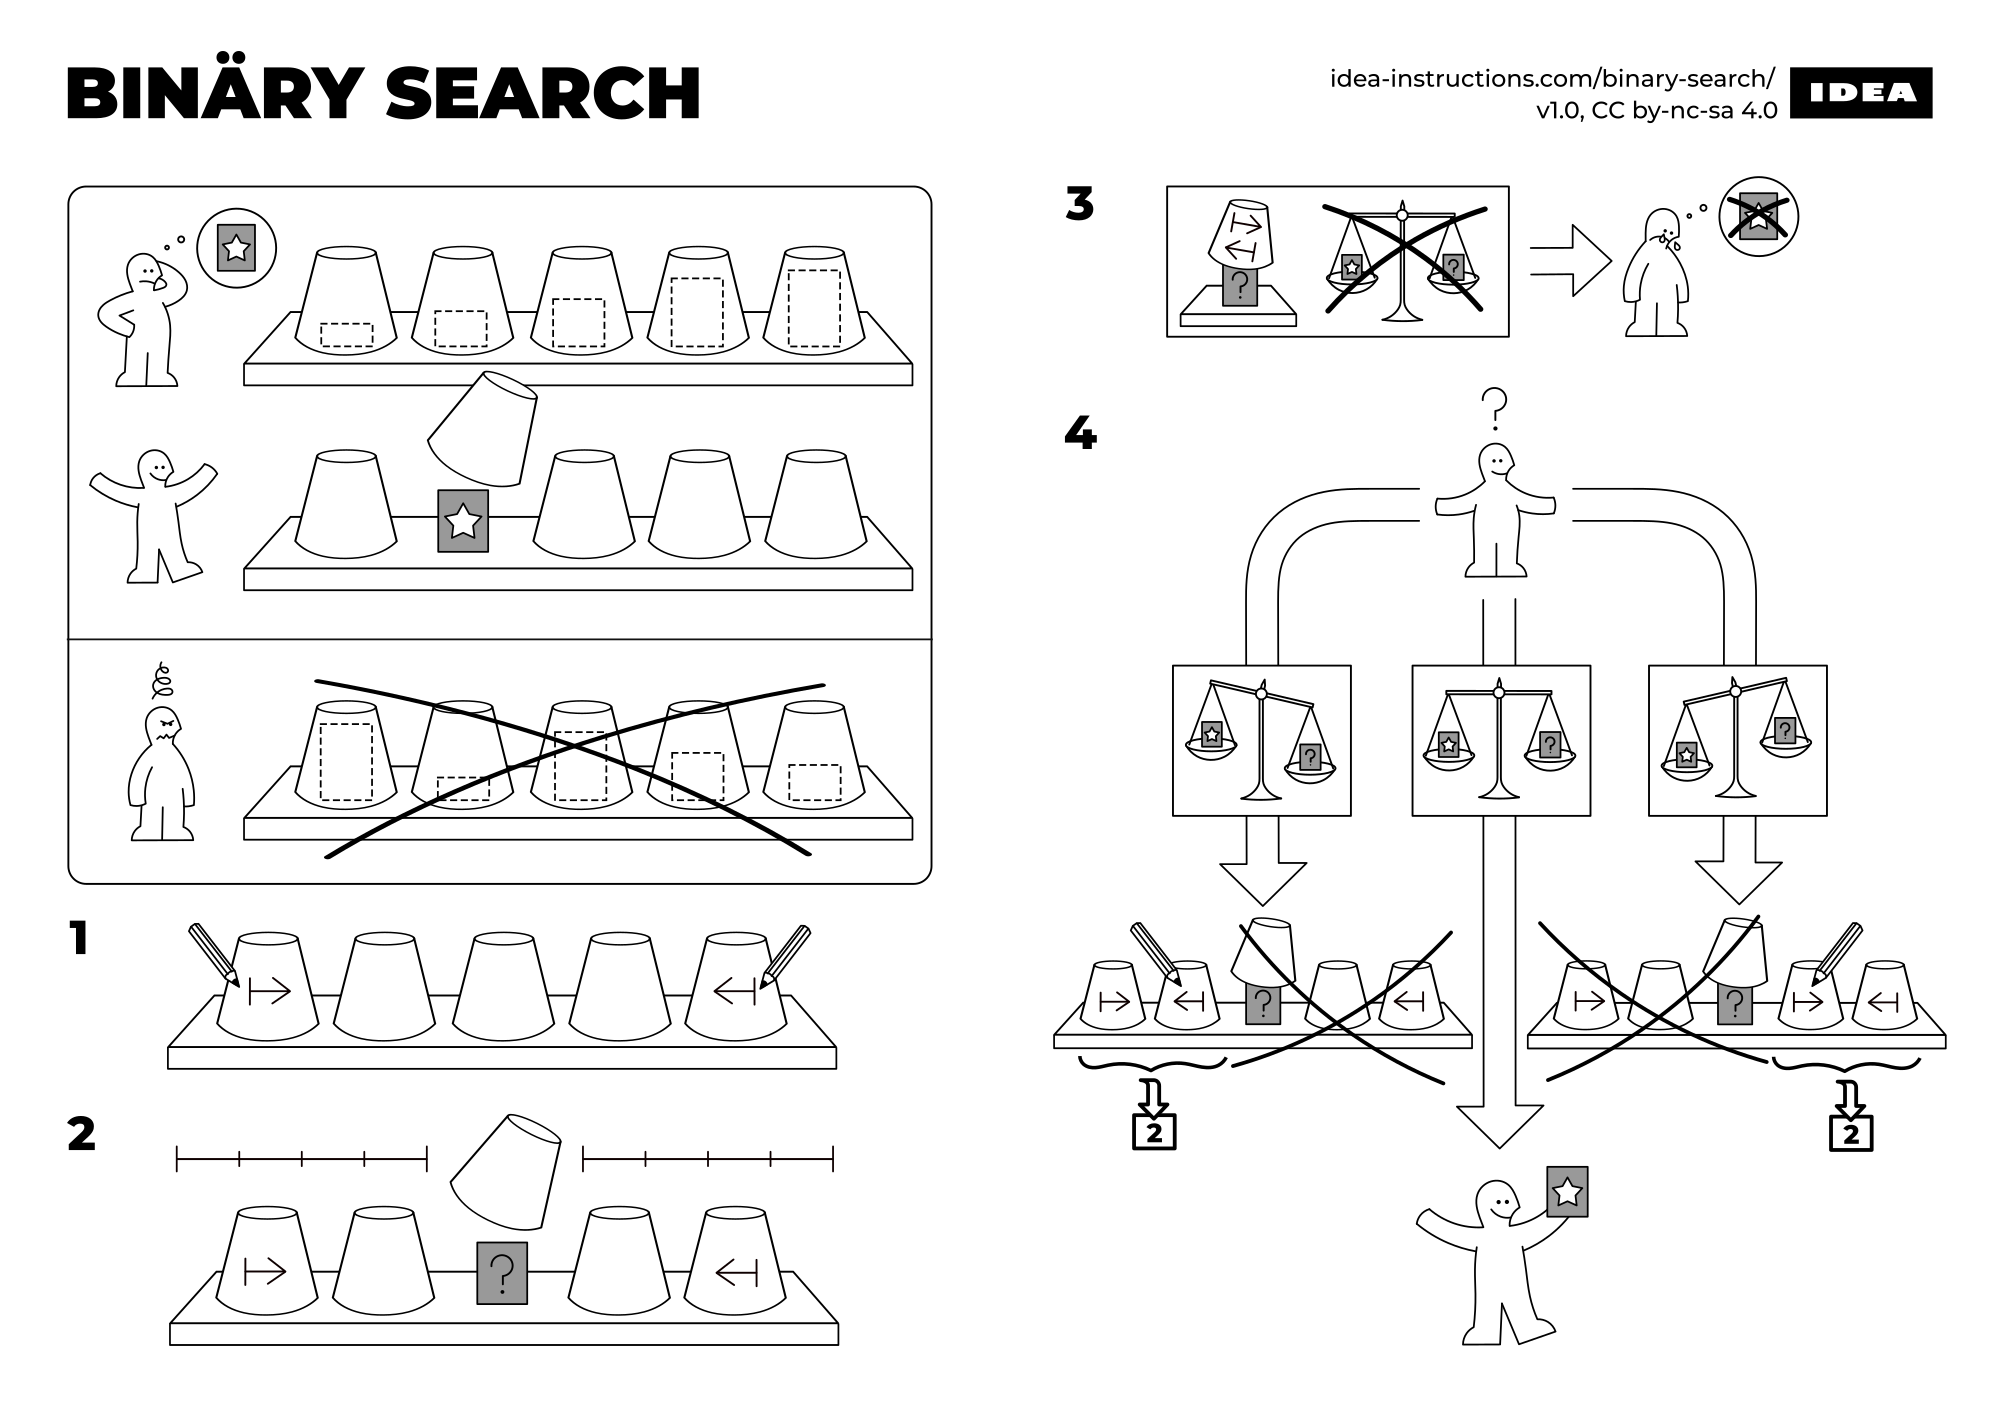
\includegraphics[width=\textwidth]{binary_search_idea}
\end{figure}